\documentclass{article}
\usepackage{amsmath, amssymb, amssymb}
\usepackage{tikz}

\begin{document}
\begin{center}
    \begin{LARGE}
        \textbf{Calculus II}
    \end{LARGE}
\end{center}

\section{Vectors}

$\mathbb{R}$ represents the set of real numbers.\\[1pt]
$\mathbb{R}^2$ represents a 2 dimensional real plane. \\[1pt]
\[\mathbb{R}^2 = \{(x,y) \mid x,y \in \mathbb{R}\}\]

%\begin{picture}

\begin{tikzpicture}
    \draw[<->] [black, ultra thin] (-3,0) -- (3,0);
    \draw[<->] [black, ultra thin] (0,-2) -- (0,2);
    \filldraw[black] (0,0) circle (1pt) node[anchor=north west] {O};
    \draw[->][black, thick] (0,0) -- (1,1) node[anchor=south west] {$(1,1)$} node[anchor=south east] {$\vec{v}$};
    \draw[->][black, thick] (0,0) -- (1,0) node[anchor=south west] {$(1,0)$} node[anchor=north] {$\vec{u}$};
    \draw[->][black, thick] (1,1) -- (1,0);
    \filldraw[black] (1,0.75) circle (0.05pt) node[anchor=west] {$\vec{v} - \vec{u}$};
\end{tikzpicture}\\[1pt]
Normally elements of $\mathbb{R}$ are known as scalers.\\[1pt]

$\cdot$ add (or subtract) two vectors

$\cdot$ if $c \in \mathbb{R}$ and $v \in \mathbb{R}^2$,  $c\vec{v}$ 

\subsection{Dot Product}
$u = (u_1, u_2)$ and $v = (v_1, v_2)$ \[u.v = u_1.v_1 + u_2.v_2\]

\subsubsection*{Theorem}
\[u.v = |u||v| \cos(\theta)\]
where $\theta$ is the angle between $\vec{u}$ and $\vec{v}$
and $|u|$ is the length of vector $\vec{u}$

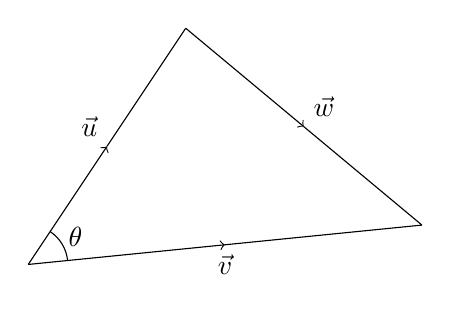
\begin{tikzpicture}
    \draw[->][black] (0,0) -- (1,1.5) node[anchor=south east] {$\vec{u}$};
    \draw [black] (1,1.5) -- (2,3);
    \draw[->] [black] (0,0) -- (2.5, 0.25) node[anchor=north] {$\vec{v}$};
    \draw [black] (2.5,  0.25) -- (5, 0.5);
    \draw[->] [black] (2,3) -- (3.5, 1.75) node[anchor=south west] {$\vec{w}$};
    \draw [black] (3.5, 1.75) -- (5, 0.5);
    \draw[black] (0.5, 0.05) arc (5.71:56.3:0.5);
    \draw[black] (0.6, 0.11) node[anchor=south] {$\theta$};
\end{tikzpicture}\\

Proof:
\[ w^2 = u^2 + v^2 - 2|u||v| \cos(\theta) \dots(1)\]
\[\vec{w} = \vec{v} - \vec{u}\]
\[ w = (v_1 - u_1, v_2 - u_2)\]
\[ w^2 = (v_1 - u_1)^2 + (v_2 - u_2)^2\]
\[ w^2 = v_1^2 - 2v_1u_1 + u_1^2 + v_2^2 - 2v_2u_2 + u_2^2\]
\[ w^2 = v^2 + u^2 - 2v_1u_1 - 2v_2u_2 \dots (2)\]

now, as $(1) = (2)$

\[ u^2 + v^2 - 2|u||v| \cos(\theta) = v^2 + u^2 - 2v_1u_1 - 2v_2u_2\]
\[|u||v| \cos(\theta) = v_1u_1 + v_2u_2\]
\[|u||v| \cos(\theta) = \vec{u}.\vec{v}\]
Hence proved.\\[1pt]

Extending the above theorem to $\mathbb{R}^n$:
Consider $\vec{u} = (u_1, u_2, \dots, u_n), \vec{v} = (v_1, v_2, \dots, v_n) \in \mathbb{R}$
\[\vec{u}.\vec{v} = u_1v_1 + u_2v_2 + \dots + u_nv_n\]

\subsection{Unit Vectors}
If $\vec{v} \in \mathbb{R}^2$ is a vector.
then, \[\hat{v} = \frac{\vec{v}}{|\vec{v}|}\]

\subsection{Projections}
If $\vec{u}$ and $\vec{v}$ are vectors in $\mathbb{R}^2$ and $\theta$ is the angle between them:

\begin{tikzpicture}
    \draw[black] (0,0) -- (2,1.5) node[anchor=south east] {$\vec{u}$};
    \draw[->] [black] (2,1.5) -- (4, 3);
    \draw[black] (0,0) -- (3, 0) node[anchor=north east] {$\vec{v}$};
    \draw[->] [black] (3,0) -- (6,0);
    \draw[black, loosely dashed] (4,3) -- (4,0);
    \draw[black] (3.8, 0) -- (3.8, 0.2);
    \draw[black] (4, 0.2) -- (3.8, 0.2);

\end{tikzpicture}

let $\vec{w}$ be the projection of $\vec{u}$ on $\vec{v}$

\[\vec{w} = |u| \cos(\theta) \hat{v}\]
\[\vec{w} = \frac{|u| \cos(\theta)|v|\vec{v} }{|v|^2}\]
\[\vec{w} = \frac{\vec{u}.\vec{v}}{|\vec{v}|^2} \vec{v}\]

\subsection{Cross Product}
Consider the vectors, $u,v$. Then the cross-product of $u$ and $v$ is defined as:
\[u \times v = |u||v|\sin(\theta) \hat{n}\]
where $\hat{n}$ is the unit vector perpendicular to the plane containing $u$ and $v$, and also $(\vec{u}, \vec{v}, \hat{n})$ form a right handed system.

\paragraph*{Properties of Cross Product: }
\begin{itemize}
    \item $\vec{u} \times \vec{v} = - (\vec{v} \times \vec{u})$
    \item $(r\vec{u}) \times (s \vec{v}) = rs \vec{u} \times \vec{v}$
    \item $ \vec{u} \times (\vec{v} + \vec{w}) = \vec{u} \times \vec{v} + \vec{u} \times \vec{w}$
\end{itemize}

$\vec{u}$ and $\vec{v}$ can also be represented as: 
\[ \vec{u} = u_1 \hat{i} + u_2 \hat{j} + u_3 \hat{k}\]
\[ \vec{v} = v_1 \hat{i} + v_2 \hat{j} + v_3 \hat{k}\]

\[\vec{u} \times \vec{v} = (u_2 v_3 - u_3 v_2)\hat{i} + (u_3 v_1 - u_1 v_3)\hat{i} + (u_1 v_2 - u_2 v_1)\hat{k}\]

\[\vec{u} \times \vec{v} = \begin{vmatrix}
    \hat{i} & \hat{j} & \hat{k} \\
    u_1 & u_2 & u_3\\
    v_1 & v_2 & v_3
\end{vmatrix}
\]
the above formula is only symbolic and meant to represent a cross product.

\section{Multi-Variable Calculus}

let $r: \mathbb{R} \rightarrow \mathbb{R}^3$ be a function.
(It could be to any $\mathbb{R}^n$)\\
for $t \in \mathbb{R}$, $r(t)$ is a vector in $\mathbb{R}^3$\\
\[r(t) = f(t)\hat{\imath} + g(t)\hat{\jmath} + h(t)\hat{k}\]

\subsection{Continuity}
$r$ is continuous at $a$ if: 
\[\lim_{t \rightarrow a} r(t) = r(a)\]
i.e. $\forall \epsilon > 0, \exists \delta > 0$ such that $|t - a| < \delta \implies |r(t) - r(a)| < \epsilon$

or, if $f$, $g$ and $h$ are continuous at $a$, $r$ is continuous at $a$.

\subsection{Differentiability}
%some random gibberish was taught

\subsection{Integration}
let $f: [a,b] \rightarrow \mathbb{R}$ be a function.\\

the integral of $f$ from $a$ to $b$ is defined as:
\[\int_a^b f(x) dx = \text{Area under the curve $y = f(x)$ from $x = a$ to $x = b$}\]

\paragraph{Anti-derivative}let $f: [a,b] \rightarrow \mathbb{R}$ be a function.\\
\[ \int f(t) dt = F(t) +c \]
such that $F'(t) = f(t)$ and $c$ is an arbitrary constant

\paragraph{Fundamental Theorem of Calculus} let $f: [a,b] \rightarrow \mathbb{R}$ be a function and $F$ be its anti-derivative.\\
\[ \int_{a}^{b} f(t) dt = F(b) - F(a) \]

\subsubsection{Extending to a Vector Valued Function}
Consider a function $r: \mathbb{R} \rightarrow \mathbb{R}^3$ (we are taking $\mathbb{R}^3$ as an example, it could be any $\mathbb{R}^n$)\\
\[ r(t) = f(t)\hat{i} + g(t)\hat{j} + h(t)\hat{k} \]
\[\int_{a}^{b}r(t)dt = \int_{a}^{b}f(t)dt\hat{i} + \int_{a}^{b}g(t)dt\hat{j} + \int_{a}^{b}h(t)dt\hat{k} \]

\paragraph{Anti-derivative}
\[ \int r(t) dt = \left(\int f(t)dt + c_1\right)\hat{i} + \left(\int g(t)dt + c_2\right)\hat{j} + \left(\int h(t)dt + c_3\right)\hat{k}  \]
\[ \int r(t) dt = R(t) + C \]
where $R'(t) = r(t)$ and $C$ is an arbitrary constant vector.
\[ R(t) = F(t)\hat{i} + G(t)\hat{j} + H(t)\hat{k} \]
where $F'(t) = f(t)$, $G'(t) = g(t)$ and $H'(t) = h(t)$



\end{document}